\documentclass[conference]{IEEEtran}
\usepackage[utf8]{inputenc}
\usepackage{amsmath,amssymb}
\usepackage{graphicx}
\usepackage{booktabs}
\usepackage{tikz}
\usetikzlibrary{arrows.meta,positioning,shapes.geometric}
\usepackage[hidelinks]{hyperref}
\usepackage{url}
\graphicspath{{figures/}}
\newcommand{\todo}[1]{\textbf{[#1]}}
\def\BibTeX{{\rm B\kern-.05em{\sc i\kern-.025em b}\kern-.08em T\kern-.1667em\lower.7ex\hbox{E}\kern-.125emX}}

\begin{document}
\title{Blind Image Restoration with Universal, Hard-Routed and Soft Mixture-of-Experts Autoencoders, and Style-Conditioned Face-to-Sketch Synthesis with a Conditional GAN}

\author{\IEEEauthorblockN{Muhammad Ruhan Kamran}
\IEEEauthorblockA{Roll No.\ 23i-0062, Section CS-A\\
AI-4009 Generative AI, Assignment \#1\\
\url{https://github.com/ruhank-dev/genai-assignment-1}\\
Demo video: \todo{YouTube link to be inserted by the author}}}
\maketitle

\begin{abstract}
We build four related generative systems and deploy them in one containerised web application. Tasks 1--3 restore Oxford-IIIT Pet images ($128\times128$) corrupted by salt-and-pepper noise, Gaussian blur or rectangular occlusion: (1) a single universal convolutional denoising autoencoder with a $3\times$ compressed latent, (2) a corruption classifier followed by three independently trained specialist autoencoders with an identity bypass (hard routing), and (3) a differentiable soft mixture-of-experts whose gate and experts are initialised from Task~2 and fine-tuned jointly. Task~4 is a style-conditioned conditional GAN (U-Net generator with FiLM style embedding, PatchGAN discriminator) for FS2K face-to-sketch synthesis. Every model is tuned with Optuna, tracked in MLflow and exported to ONNX (maximum PyTorch/ONNX Runtime deviation $1.9\times10^{-5}$). On the official test set, the mean PSNR/SSIM over the nine corrupted variants is 23.70\,dB/0.782 (Task~1), 24.23\,dB/0.790 (Task~2, predicted routing) and 24.73\,dB/0.819 (Task~3); the classifier reaches 99.65\% accuracy; the face-to-sketch generator obtains L1 0.100, SSIM 0.498 and FID 102.1 on 1\,046 test pairs. We discuss failure modes, routing behaviour and limitations of each system.
\end{abstract}

\begin{IEEEkeywords}
denoising autoencoder, mixture of experts, conditional GAN, Optuna, ONNX, FastAPI, Docker
\end{IEEEkeywords}

\section{Introduction}
Image restoration systems are normally evaluated on one degradation at a time, yet deployed models see unknown mixtures of degradations. This work studies three architectures for \emph{blind} restoration of three corruption families---impulsive noise, low-pass blur and large missing regions---and a fourth, generative problem: converting a face photograph into a sketch in one of three artistic styles. The goal is not only accuracy but a complete, reproducible pipeline: data preparation with deterministic corruption manifests, hyper-parameter optimisation (Optuna), experiment tracking (MLflow), export (ONNX) and a browser application (React, FastAPI, Docker Compose) through which an evaluator can upload images, corrupt them at run time, inspect classifier probabilities and gate weights, and download generated sketches.

\textbf{Contributions.} (i) A controlled comparison of universal, hard-routed and soft-routed restoration on identical data, manifests and metrics. (ii) A routing analysis that shows the soft gate learns \emph{severity-aware} blending. (iii) A reproducible style-conditioned GAN with a measured comparison of conditioning mechanisms and discriminator receptive fields. (iv) Honest reporting of failures, null results and every deviation from the planned experimental budget.

\section{Related Work}
Denoising autoencoders learn to reconstruct a clean signal from a corrupted input through a bottleneck~\cite{vincent2008}; U-Net style skip connections~\cite{ronneberger2015} improve detail but let information bypass the latent, which we avoid in Task~1. Structural similarity~\cite{wang2004} complements pixel losses with local luminance/contrast/structure terms. Mixtures of experts combine specialists through a learned gate~\cite{shazeer2017}; load-balancing regularisers prevent routing collapse~\cite{shazeer2017,fedus2021}. Image-to-image translation with conditional GANs and PatchGAN discriminators~\cite{mirza2014,isola2017} is the basis of Task~4; feature-wise linear modulation (FiLM)~\cite{perez2018} injects a conditioning vector into feature maps. Hyper-parameter search uses Optuna's TPE sampler and median pruner~\cite{akiba2019}; generated images are evaluated with LPIPS~\cite{zhang2018} and FID~\cite{heusel2017}.

\section{Datasets and Corruption Pipeline}
\textbf{Oxford-IIIT Pet}~\cite{parkhi2012} (37 breeds). The official \texttt{trainval} set (3\,680 images) is split 80/20 with seed 42, stratified by breed, into 2\,944 training and 736 validation images; the 3\,669-image official test set is untouched until final evaluation. Images are converted to RGB, resized to $128\times128$ (bicubic) and scaled to $[0,1]$.

\textbf{Corruptions} (Table~\ref{tab:corr}, Fig.~\ref{fig:corr}). During training one of four conditions (clean, salt-and-pepper, blur, occlusion) is drawn with equal probability and with random parameters every time an image is loaded, inside the data loader; the label is kept for the classifier. Validation (736 entries, exactly 25\% per type) and test (10 variants $\times$ 3\,669 images $=$ 36\,690 entries) corruptions are generated once and stored as JSON manifests of parameters (type, severity, mask coordinates, blur settings, seed). For occlusion, rectangles are placed by a best-of-40 least-overlap rule so that the realised area matches the target (mean coverage 9.99/19.98/34.95\% for the three levels over 200 draws; random placement alone under-covered the 3-box case at 28.8\%).

\begin{table}[t]\centering\caption{Corruption configuration.}\label{tab:corr}\small
\resizebox{\columnwidth}{!}{\begin{tabular}{@{}lll@{}}\toprule
Condition & Training & Test severities (low/med/high)\\\midrule
Salt-and-pepper & $p\sim U(0.02,0.15)$ & $p=0.03,\,0.08,\,0.15$\\
Gaussian blur & $k\in\{3,5,7\},\ \sigma\sim U(0.5,2.5)$ & $(3,0.7),(5,1.5),(7,2.5)$\\
Occlusion (black) & 1--3 boxes, 10--35\% area & 1/2/3 boxes, $\approx$10/20/35\%\\\bottomrule
\end{tabular}}\end{table}
\begin{figure}[t]\centering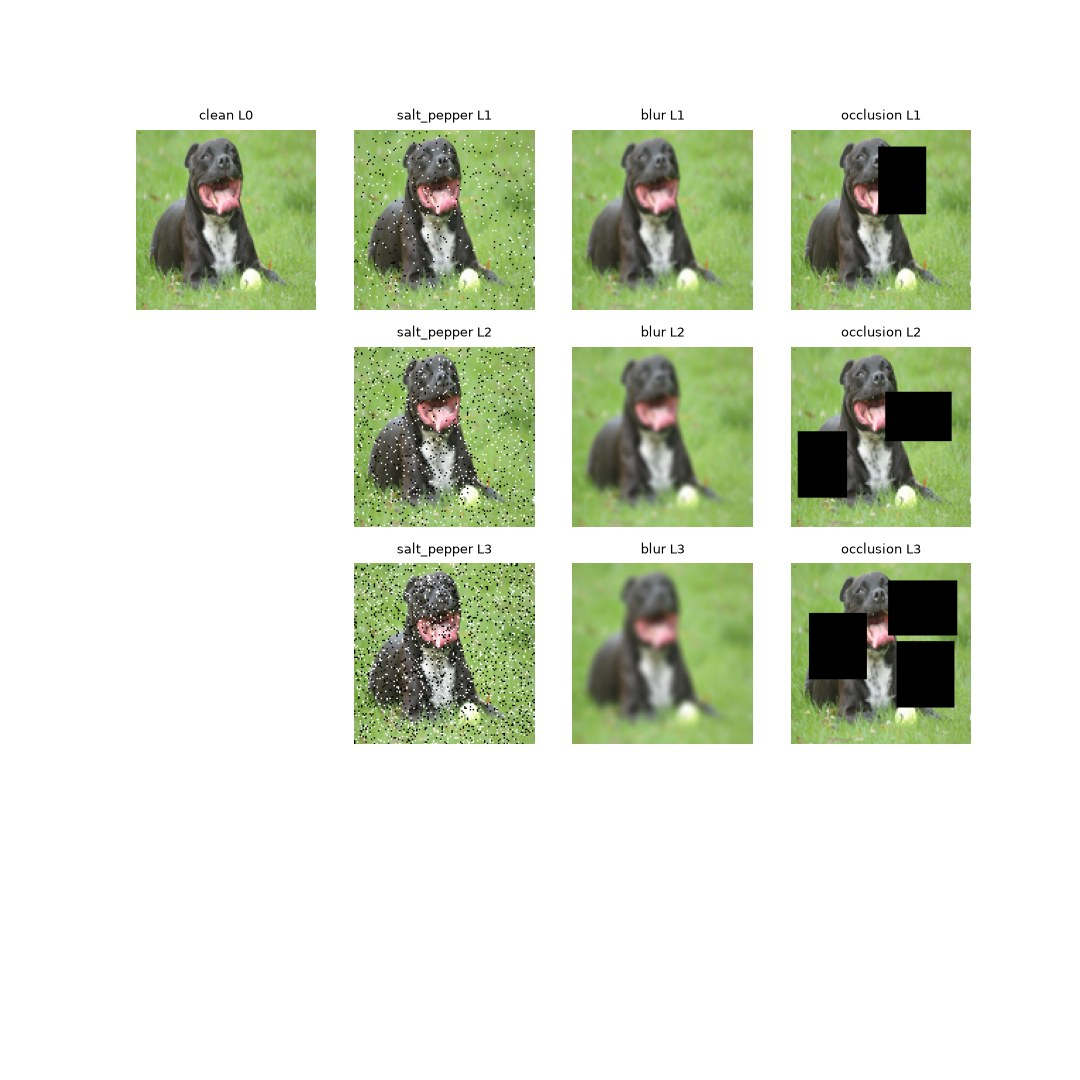
\includegraphics[width=0.78\columnwidth]{corruption_grid.jpg}\caption{Clean image and the three severities of each corruption (test levels).}\label{fig:corr}\end{figure}

\textbf{FS2K}~\cite{fan2022}. 2\,104 photograph--sketch pairs with three sketch styles. We use the official split (1\,058 train / 1\,046 test) and reserve 15\% of the training part, stratified by style (seed 42), as validation: 899 train / 159 validation pairs (style counts 303/298/298 and 54/52/53; test 619/381/46). Photos and sketches are resized to $128\times128$ and scaled to $[-1,1]$. Every pair is verified at indexing time.

\textbf{Metrics.} PSNR ($\mathrm{MAX}=1$, $\epsilon=10^{-8}$, hence exact copies are capped at 80\,dB), SSIM (Gaussian $11\times11$ window, $\sigma=1.5$) and mean absolute error (L1). Because the identity bypass reproduces clean inputs exactly, we additionally report the mean over the nine \emph{corrupted} test variants.

\section{Task 1: Universal Denoising Autoencoder}
\subsection{Architecture and loss}
The encoder halves the spatial size at every stage while widening channels (each stage: strided conv, conv, BatchNorm, LeakyReLU), followed by a $1\times1$ projection to a bottleneck and Dropout2d; the decoder mirrors it with bilinear up-sampling and convolutions (avoiding checkerboard artefacts) and a final $1\times1$ conv with Sigmoid. There are \emph{no} skip connections, so the latent is a genuine bottleneck. The loss is $\mathcal{L}=\alpha\mathcal{L}_1(x,\hat x)+(1-\alpha)(1-\mathrm{SSIM}(x,\hat x))$ with $\hat x=D(E(\tilde x))$. A 5-epoch experiment on 15\% of the data ($\alpha\in\{0,0.5,0.8,1\}$, validation $L_1+(1-\mathrm{SSIM})$: 0.801/0.770/0.775/0.780; PSNR 14.1/15.1/15.3/15.4\,dB) showed pure SSIM is worst everywhere and pure L1 gives the best PSNR; with only 5 epochs the differences among $\alpha\ge0.5$ are small, so $\alpha$ is left to Optuna. Mixed-precision (fp16) training stalled learning on our GPU (loss $0.354\to0.335$ vs.\ $0.354\to0.118$ in 150 steps in fp32), so all models are trained in fp32.

\subsection{Hyper-parameter optimisation}
The Optuna study searches learning rate ($10^{-4}$--$10^{-2}$, log), batch size $\{16,32,64\}$, bottleneck channels $\{64,128,256,512\}$, encoder widths (three configurations), dropout (0--0.5) and $\alpha$ (0.5--1) with TPE (seed 42) and a median pruner (SQLite storage). The objective is $L_1+(1-\mathrm{SSIM})$ on the validation manifest, which is independent of $\alpha$ so that trials are comparable. A first, unconstrained 16-trial study converged to a 512-channel latent on $16\times16$ maps, i.e.\ a latent $2.7\times$ \emph{larger} than the input---not a bottleneck. We therefore added the constraint \emph{input values/latent values $\ge2$} (infeasible trials are skipped untrained). In the constrained study (12 trained trials of 20 epochs; 8 completed, 4 pruned) the best trial (objective 0.3239) uses lr $1.81\times10^{-3}$, batch 32, bottleneck 64 on $16\times16$ maps (compression $3.0\times$), widths $[32,64,128]$, dropout 0.369 and $\alpha=0.509$. The final model (517\,683 parameters) is retrained for 80 epochs (cosine schedule): validation PSNR 24.38\,dB, SSIM 0.802 (baseline: 22.88\,dB, 0.679; Fig.~\ref{fig:t1curves}). An earlier final run that early-stopped at epoch 35, before the cosine schedule annealed, scored only 21.31\,dB overall on the test set (versus 23.87\,dB), so the schedule is run to completion.

\begin{figure}[t]\centering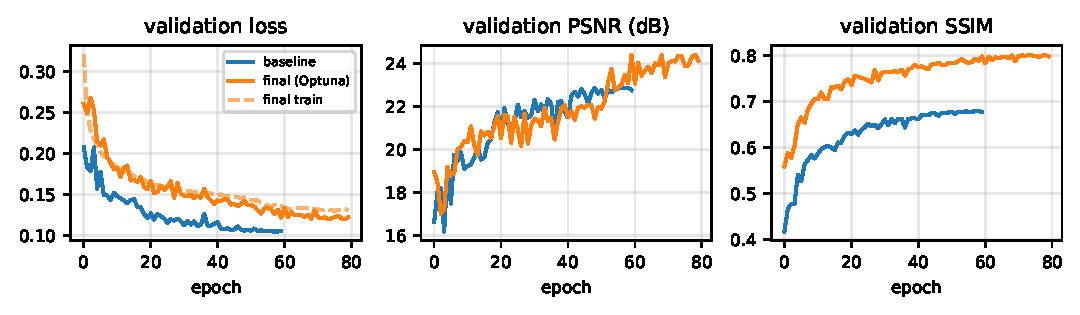
\includegraphics[width=\columnwidth]{t1_curves.pdf}\caption{Task 1 validation curves: baseline (60 epochs) vs.\ Optuna configuration (80 epochs).}\label{fig:t1curves}\end{figure}

\subsection{Results}
Table~\ref{tab:t1} gives test results per corruption and severity (36\,690 manifest samples). Overall: 23.87\,dB, SSIM 0.788, L1 0.0479 (0.50\,ms/sample on GPU). Clean and salt-and-pepper inputs are restored almost equally well (25.3\,dB; the clean ceiling is set by the bottleneck, not by noise), mild blur costs nothing and strong blur costs 1.5\,dB, whereas occlusion is clearly hardest and degrades monotonically with area (22.8$\to$19.3\,dB).

\begin{table}[t]\centering\caption{Task 1 test results (PSNR dB / SSIM / L1).}\label{tab:t1}\small
\resizebox{\columnwidth}{!}{\begin{tabular}{@{}llccc@{}}\toprule
Condition & Severity & PSNR & SSIM & L1\\\midrule
Clean & -- & 25.35 & 0.839 & 0.0415\\
Salt-pepper & low/med/high & 25.32/25.19/24.87 & 0.836/0.828/0.813 & 0.042/0.042/0.044\\
Blur & low/med/high & 25.47/25.28/23.89 & 0.834/0.818/0.733 & 0.041/0.042/0.048\\
Occlusion & low/med/high & 22.82/21.18/19.28 & 0.786/0.735/0.656 & 0.050/0.058/0.071\\\bottomrule
\end{tabular}}\end{table}
\begin{figure}[t]\centering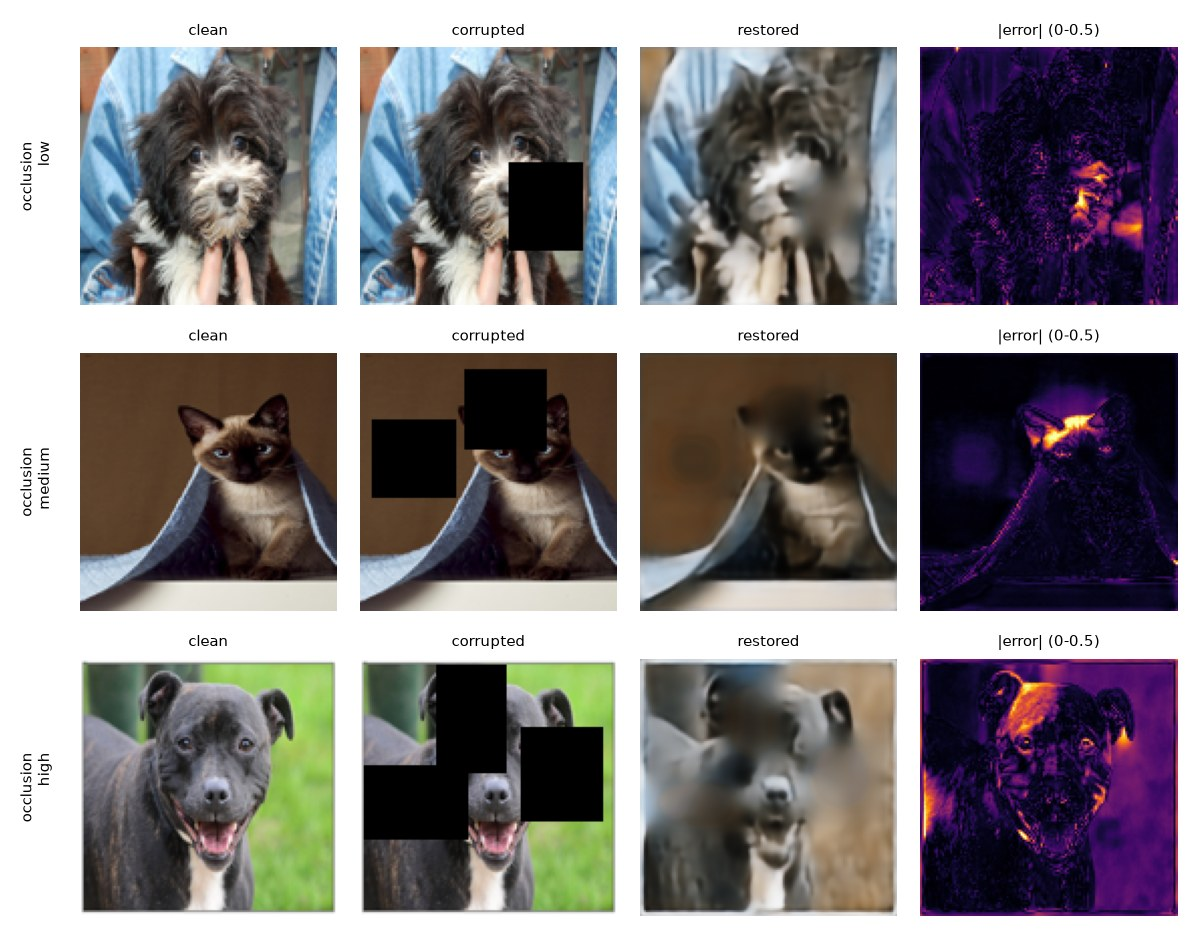
\includegraphics[width=\columnwidth]{t1_examples_occ.jpg}\caption{Task 1: clean target, occluded input, reconstruction and absolute error map (fixed scale 0--0.5) for low/medium/high occlusion. Twelve representative examples (three per condition) are in the repository results.}\label{fig:t1ex}\end{figure}
\textbf{Failure cases.} Four failures were analysed (worst PSNR for high occlusion 12.1\,dB, high salt-and-pepper 14.8\,dB, high blur 14.4\,dB, and the lowest-SSIM occlusion, SSIM 0.34; Fig.~\ref{fig:t1fail}). With three boxes hiding most of an animal on a busy yellow-flower meadow, the whole background is rebuilt as orange-brown texture: the $3\times$ compressed latent cannot represent high-frequency backgrounds, and L1/SSIM objectives favour averaged, blurry content. The same fur-textured image fails under both strong blur and strong noise, where fine detail is irrecoverable.
\begin{figure}[t]\centering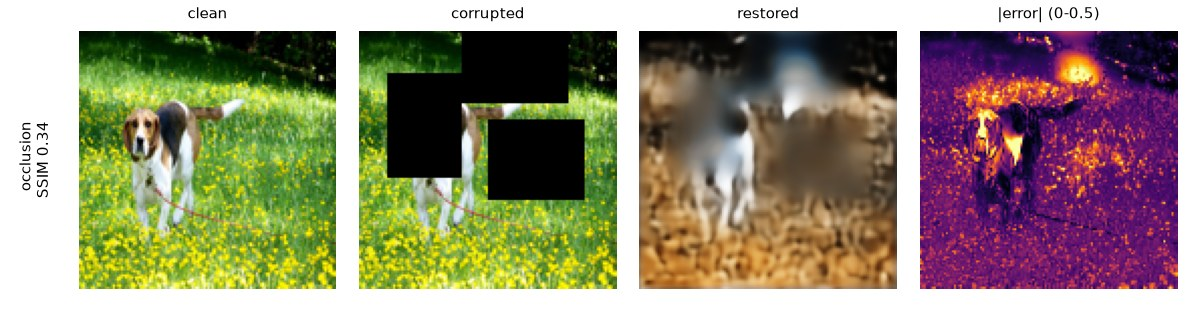
\includegraphics[width=0.95\columnwidth]{t1_failure.jpg}\caption{Task 1 failure case: three occlusion boxes on a high-frequency meadow background.}\label{fig:t1fail}\end{figure}

\section{Task 2: Corruption Classifier and Hard-Routed Specialists}
\textbf{Pipeline.} A classifier $C$ predicts $r=\arg\max_k p_k$ over (clean, salt-and-pepper, blur, occlusion); $r=0$ uses an exact identity bypass, otherwise the corresponding specialist $A_r$ restores the image. Batches are grouped by route so each expert runs once per batch.

\textbf{Classifier.} Training batches are exactly class-balanced ($B/4$ per class). In a 3-epoch comparison all candidates exceeded 99.4\% validation macro-F1: custom conv stacks with 72\,K/288\,K/1.17\,M parameters (F1 0.9973/0.9973/0.9946; 1.7/1.7/2.1\,ms) and ImageNet-pretrained ResNet-18 (11.2\,M parameters; F1 0.9986; 4.75\,ms). We chose the custom conv stack (two conv-BN-ReLU per stage, max-pool, global average pooling, dropout, linear head): ResNet-18 gains 0.13 points for 40$\times$ the parameters. An Optuna study (learning rate, batch size, channel configuration, dropout, weight decay; 12 trials $\times$ 5 epochs, 6 pruned) saturated at 0.997 macro-F1 for several settings (differences of one to three validation images), selecting channels $[32,\dots,256]$, lr $7.3\times10^{-4}$, dropout 0.4. The final model (15 epochs) reaches 99.86\% validation accuracy. On the test manifest: accuracy 0.9965, macro precision/recall/F1 0.9966/0.9919/0.9942 (Fig.~\ref{fig:conf}); salt-and-pepper is perfect, while 114 of 3\,669 clean images are routed to the blur (80) or occlusion (34) specialists.
\begin{figure}[t]\centering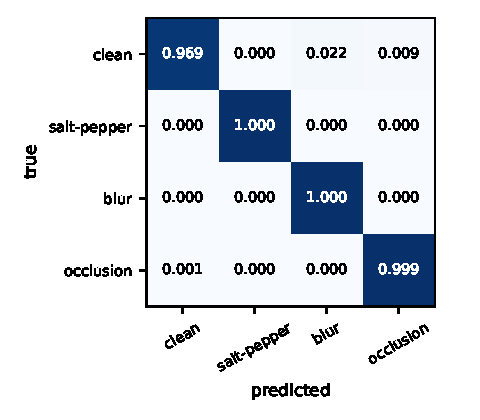
\includegraphics[width=0.62\columnwidth]{t2_confusion.pdf}\caption{Task 2 classifier: normalised confusion matrix on the test manifest.}\label{fig:conf}\end{figure}

\textbf{Specialists.} The three specialists reuse the Task~1 topology with independent weights and are each trained only on their own corruption with the clean image as target. One shared Optuna search on the mixed salt/blur/occlusion validation manifest (12 trained trials $\times$ 10 epochs, compression $\ge2\times$) selects channels $[32,64,128]$, bottleneck 64, lr $5.6\times10^{-4}$, batch 16, $\alpha=0.5$. Compared with Task~1-baseline-configured specialists (25 epochs: 23.07/23.20/19.43\,dB for salt/blur/occlusion), the final specialists (40 epochs) reach 25.63/26.16/21.52\,dB (SSIM 0.827/0.837/0.726) on their validation sets.

\textbf{Oracle vs.\ predicted routing.} Table~\ref{tab:t2} compares Task~1, oracle routing (true label from the manifest) and predicted routing on the test set. Specialists beat the universal autoencoder at every corrupted severity (+0.2 to +0.8\,dB). Because the classifier is nearly perfect, the oracle--predicted gap on corrupted inputs is $<0.02$\,dB; the entire practical loss lies in clean images that are misrouted (127 of 36\,690 samples misrouted overall, 0.35\%). The worst cases (Fig.~\ref{fig:mis}): a clean cat on a pure black background is classified as occluded (black regions resemble masks) and its occlusion specialist \lq inpaints\rq\ the background (80$\to$11.2\,dB); clean$\to$blur over-smooths (80$\to$17.1\,dB); an occluded image routed to the blur expert cannot be filled (28.2$\to$17.3\,dB); a false clean bypass of a small box only costs 1\,dB. Hard routing doubles the per-sample cost (0.91 vs.\ 0.50\,ms) because of the classifier pass.
\begin{table}[t]\centering\caption{Task 2 test PSNR (dB) by condition.}\label{tab:t2}\small
\resizebox{\columnwidth}{!}{\begin{tabular}{@{}lccc@{}}\toprule
Condition (low/med/high) & Task 1 & Oracle & Predicted\\\midrule
Salt-pepper & 25.3/25.2/24.9 & 25.6/25.5/25.3 & 25.6/25.5/25.3\\
Blur & 25.5/25.3/23.9 & 25.9/26.1/24.7 & 25.9/26.1/24.7\\
Occlusion & 22.8/21.2/19.3 & 23.3/21.8/20.0 & 23.3/21.8/20.0\\
Clean & 25.35 & 80.0$^\ast$ & 78.3$^\ast$\\\midrule
Mean, 9 corrupted variants & 23.70 / 0.782 & 24.22 / 0.790 & 24.23 / 0.790\\\bottomrule
\multicolumn{4}{@{}l}{\footnotesize $^\ast$exact identity bypass (PSNR capped at 80\,dB); SSIM in last row.}
\end{tabular}}\end{table}
\begin{figure}[t]\centering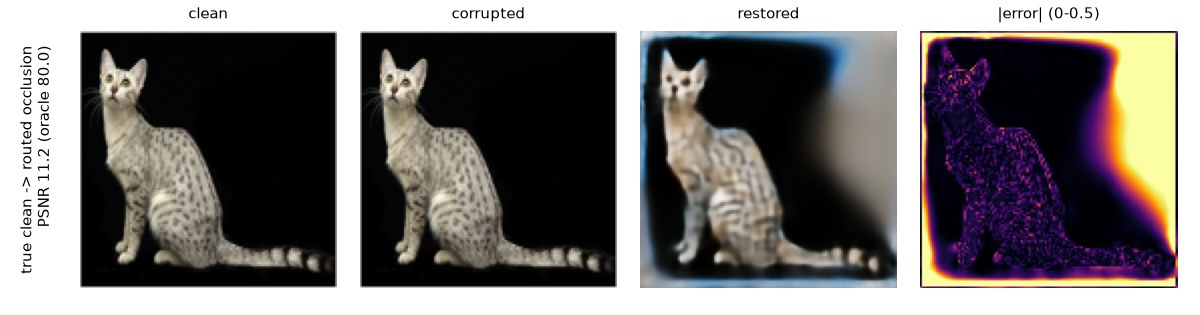
\includegraphics[width=0.95\columnwidth]{t2_misroute.jpg}\caption{Largest misrouting failure: a clean image routed to the occlusion specialist.}\label{fig:mis}\end{figure}

\section{Task 3: Jointly Trained Soft Mixture-of-Experts}
\textbf{Model.} $w=\mathrm{softmax}(G(\tilde x)/\tau)$ and $\hat x=w_1\tilde x+w_2A_\text{salt}(\tilde x)+w_3A_\text{blur}(\tilde x)+w_4A_\text{occ}(\tilde x)$, where $G$ is the Task~2 classifier (convolutional features, global pooling, linear head) copied one-to-one and the experts are the Task~2 specialists; $\tau$ is clamped to $\ge0.05$. The identity branch has no parameters. The loss is $\lambda_1\mathcal{L}_1+\lambda_2(1-\mathrm{SSIM})+\lambda_3\mathrm{CE}(z,y)+\lambda_4\mathcal{L}_\text{bal}(w)$ with initial weights 0.8/0.2/0.1/0.01 and $\mathcal{L}_\text{bal}=\sum_k(\bar w_k-1/4)^2$ over class-balanced batches. Training has a gate-only warm-up with frozen experts (verified bit-exact against the Task~2 checkpoints) followed by joint fine-tuning with a smaller learning rate (experts $\eta$, gate $5\eta$).

\textbf{Design experiments.} A linear versus MLP gate head (3 epochs) gave validation SSIM 0.8482 vs.\ 0.8537, within noise, so the linear gate is used. The L2, negative-entropy and Switch-style balance regularisers (3+7 epochs each) gave identical results (SSIM 0.848, routing uniform at 0.25 $\pm$0.003, no collapse): with an accurate gate and class-balanced batches the batch-mean routing is already uniform, so the experiment cannot discriminate between them; the assignment's L2 form is kept. In these first runs validation SSIM \emph{fell} during the joint phase (0.848$\to$0.841). Because every expert sees all corruption types inside the MoE forward pass, its BatchNorm statistics drifted; keeping expert BatchNorm in evaluation mode during joint training fixed this (baseline run: corrupted-only validation PSNR 24.47$\to$24.68\,dB, SSIM 0.8481$\to$0.8489).

\textbf{Optuna.} 10 trials (2 warm-up + 6 joint epochs; 7 completed, 3 pruned, none collapse-pruned) over joint learning rate, $\tau$, $\lambda_3$, $\lambda_4$ and the L1/SSIM weight $\alpha$ with the objective of maximum validation SSIM. Best (SSIM 0.8642 vs.\ baseline 0.8489): $\eta=1.75\times10^{-5}$, $\tau=2.53$, $\lambda_3=0.0114$, $\lambda_4=0.0659$, $\alpha=0.629$. Final retraining (10 warm-up + 40 joint epochs) reaches validation SSIM 0.8676.

\textbf{Routing behaviour.} Table~\ref{tab:route} lists the mean gate weights per true corruption (test) and Fig.~\ref{fig:heat}--\ref{fig:trend} show them per severity. Each expert is used mainly for its own corruption, and the weight of the matching expert rises with severity (salt: 0.868$\to$0.947$\to$0.977; blur 0.584$\to$0.829$\to$0.890; occlusion 0.417$\to$0.742$\to$0.915) while the identity share falls: the gate learned that mild corruption needs only partial restoration. 60.1\% of test samples have a dominant expert ($w_{\max}>0.85$); 12.7\% have $w_{\max}<0.6$ (e.g.\ low-severity noise split 0.45/0.45 between identity and the salt expert; Fig.~\ref{fig:soft}). No expert is inactive (overall mean weights 0.26/0.28/0.24/0.22). The salt and blur experts never dominate unrelated inputs ($\le0.1\%$), but the identity branch dominates 26.1\% of occluded inputs (small boxes).
\begin{table}[t]\centering\caption{Task 3: mean gate weights by true corruption (test).}\label{tab:route}\small
\begin{tabular}{@{}lcccc@{}}\toprule
True & identity & salt & blur & occlusion\\\midrule
Clean & 0.894 & 0.000 & 0.016 & 0.089\\
Salt-pepper & 0.043 & 0.931 & 0.024 & 0.002\\
Blur & 0.218 & 0.000 & 0.768 & 0.014\\
Occlusion & 0.307 & 0.000 & 0.002 & 0.691\\\bottomrule
\end{tabular}\end{table}
\begin{figure}[t]\centering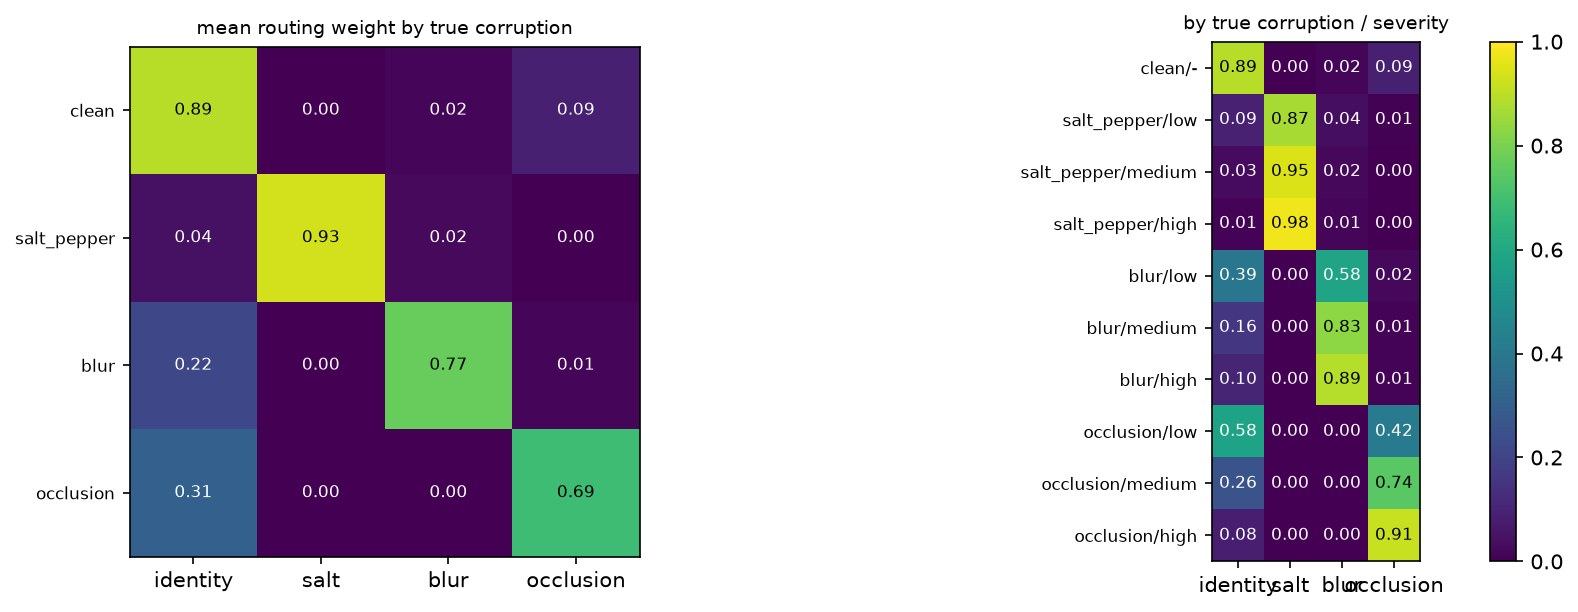
\includegraphics[width=\columnwidth]{t3_heatmap.jpg}\caption{Routing heat-map: mean weights per true corruption and per corruption/severity.}\label{fig:heat}\end{figure}
\begin{figure}[t]\centering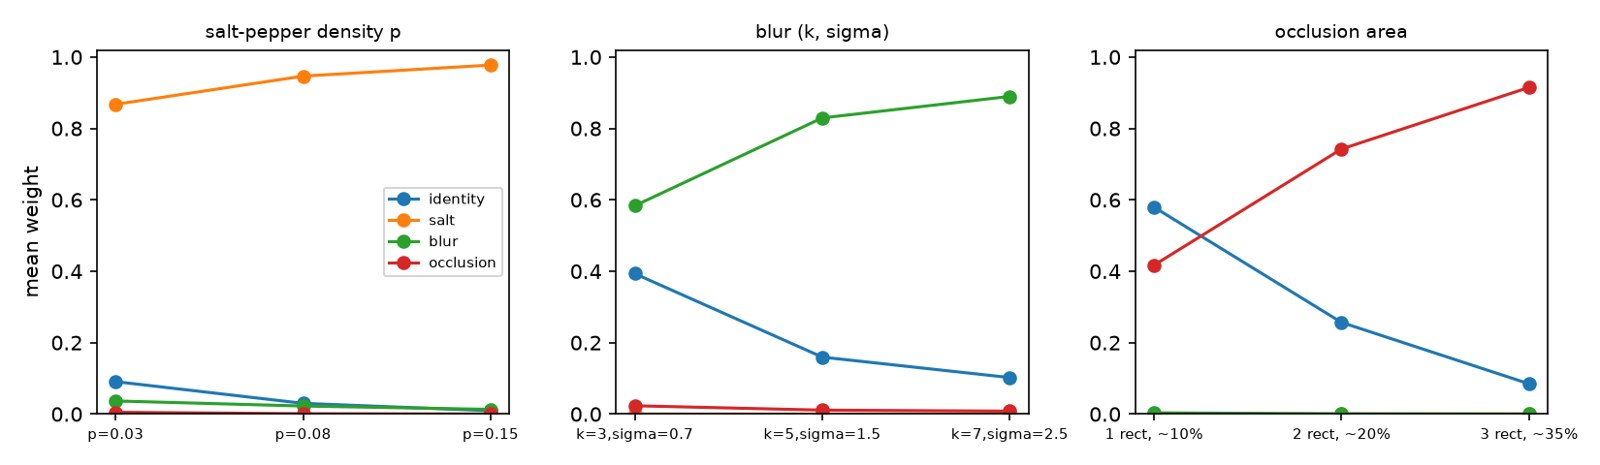
\includegraphics[width=\columnwidth]{t3_trends.jpg}\caption{Gate weights as corruption severity increases.}\label{fig:trend}\end{figure}
\begin{figure}[t]\centering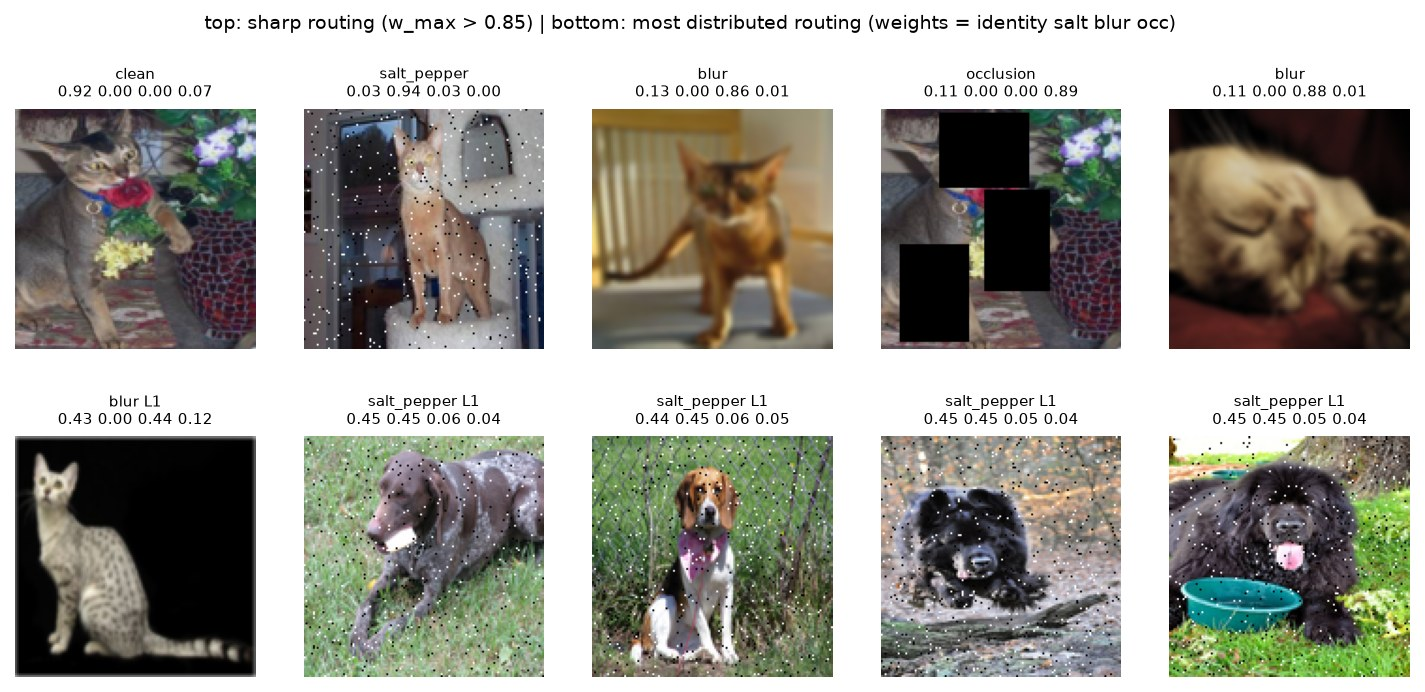
\includegraphics[width=\columnwidth]{t3_sharp_soft.jpg}\caption{Top: sharp routing ($w_{\max}>0.85$). Bottom: most distributed routing. Weights are ordered identity, salt, blur, occlusion.}\label{fig:soft}\end{figure}

\textbf{Comparison.} Table~\ref{tab:cmp} summarises the three restoration systems on the test set. The soft MoE achieves the best corrupted-only PSNR/SSIM (24.73\,dB/0.819) and wins on salt-and-pepper (+0.5 to +1.1\,dB over Task~2) and blur (+2.8\,dB at low severity). It loses on low-severity occlusion (21.48 vs.\ 23.27\,dB) because the 0.58 identity weight re-inserts the black box into the blend, and it cannot reproduce clean images exactly (46.4\,dB vs.\ an exact copy). It is more robust to classifier mistakes: on the 127 images Task~2 misrouted, Task~3 has higher PSNR on 95.3\% (e.g.\ a clean image sent to the blur expert: 19.1\,dB vs.\ 46.7\,dB with weights $[0.958,0,0.006,0.036]$). Its cost is 1.93\,ms/sample since all branches run. A caveat: Task~3 was tuned on validation SSIM with $\alpha=0.63$, which partly explains its SSIM lead.
\begin{table}[t]\centering\caption{Test comparison (mean over the nine corrupted variants).}\label{tab:cmp}\small
\begin{tabular}{@{}lccc@{}}\toprule
Method & PSNR (dB) & SSIM & ms/sample\\\midrule
Task 1 universal AE & 23.70 & 0.782 & 0.50\\
Task 2 hard (predicted) & 24.23 & 0.790 & 0.91\\
Task 2 hard (oracle) & 24.22 & 0.790 & 0.91\\
Task 3 soft MoE & \textbf{24.73} & \textbf{0.819} & 1.93\\\bottomrule
\end{tabular}\end{table}
\begin{figure}[t]\centering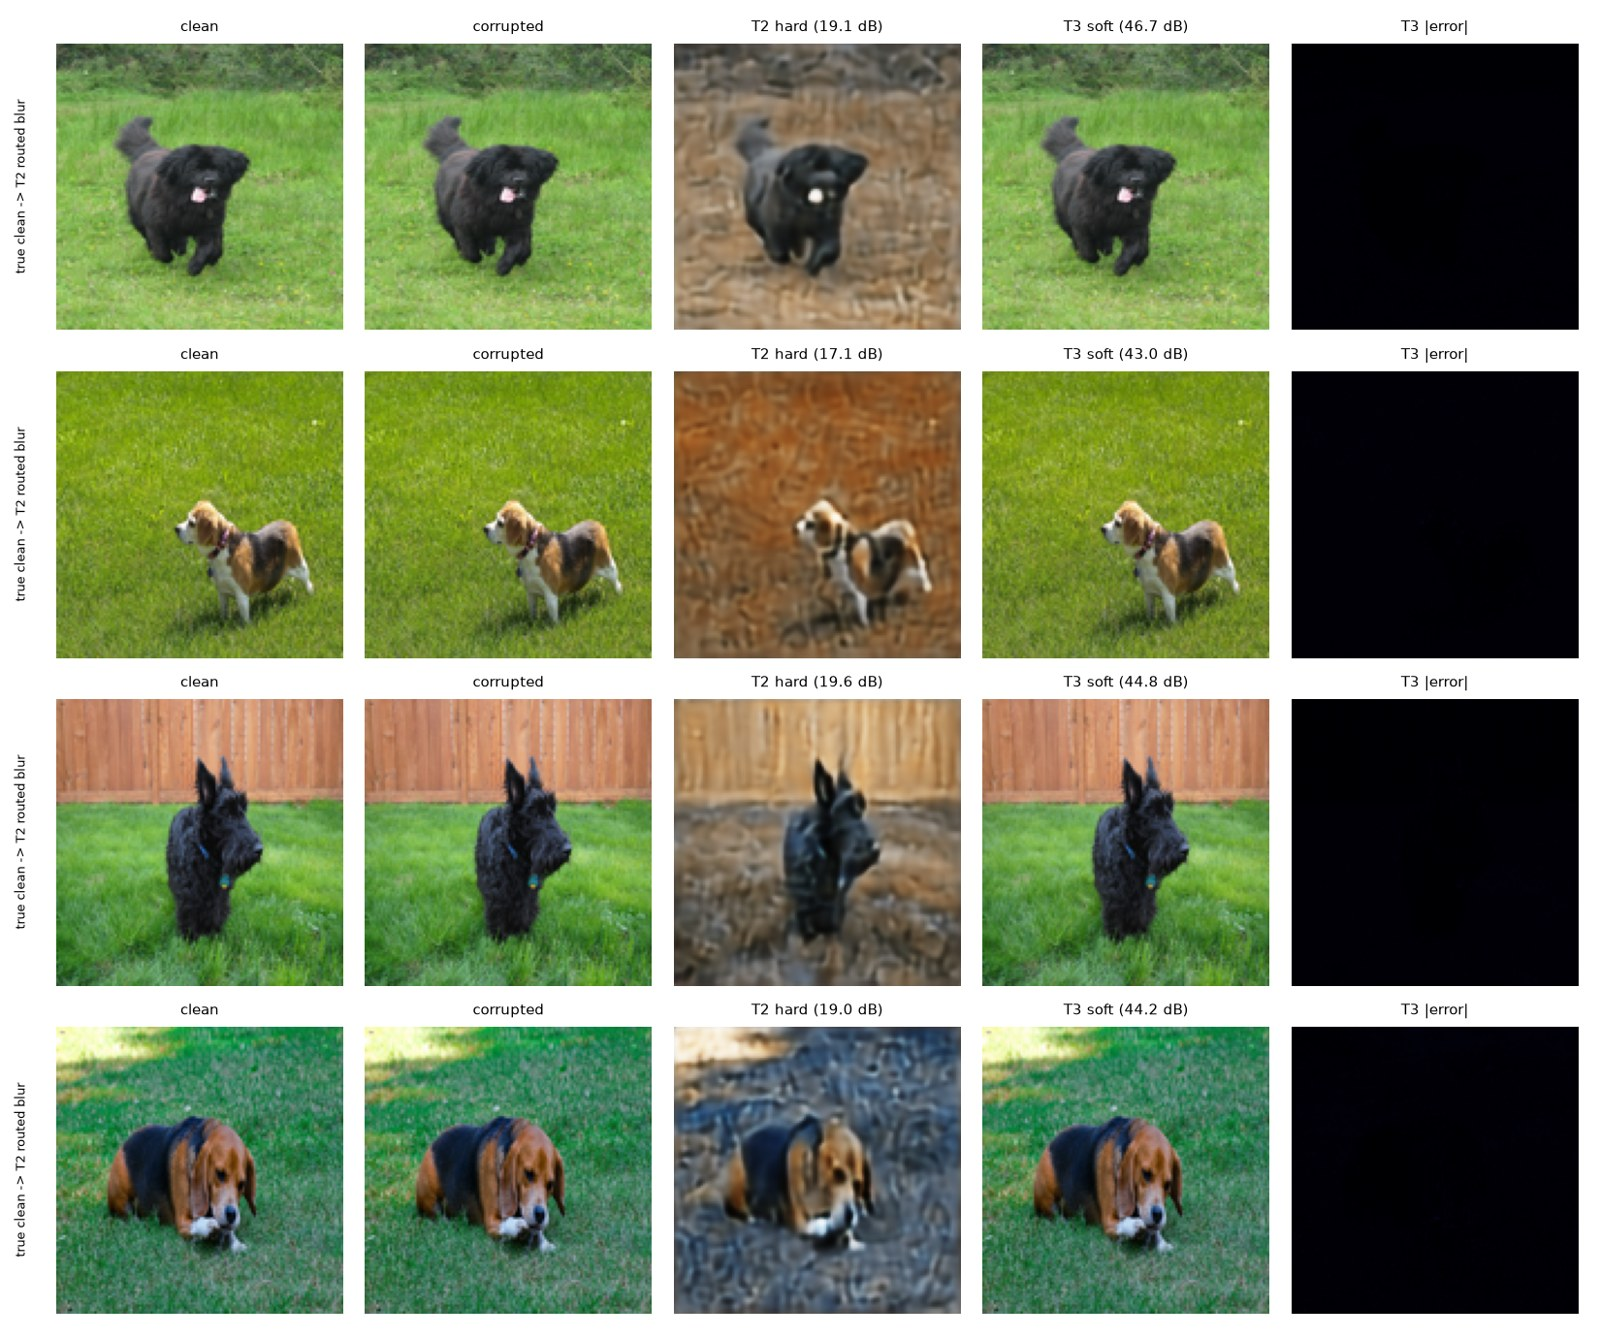
\includegraphics[width=\columnwidth]{t3_recovery.jpg}\caption{Task~2 misroutes (left to right: clean, corrupted, hard-routed, soft MoE, soft-MoE error) that the soft MoE handles.}\label{fig:rec}\end{figure}

\section{Task 4: Style-Conditioned Face-to-Sketch cGAN}
\textbf{Model.} The generator $G(x,s)$ is a pix2pix-style U-Net (five stride-2 stages $128\to4$, skip connections, InstanceNorm, Tanh; 19.1\,M parameters at base width 64) with a learned embedding $e_s\in\mathbb{R}^{d_s}$ that modulates every decoder block through FiLM ($\gamma(s),\beta(s)$ from $e_s$; zero-initialised so training starts as a plain U-Net) and is concatenated at the bottleneck. The discriminator $D(x,y,s)$ is a conditional PatchGAN over the concatenation of photo, sketch and the spatially replicated style embedding of its own, so the style enters both networks. Losses use BCE with logits: $\mathcal{L}_D=\tfrac12[\mathrm{BCE}(D(x,y,s),0.9)+\mathrm{BCE}(D(x,G(x,s),s),0)]$ (one-sided label smoothing), $\mathcal{L}_G=\mathrm{BCE}(D(x,G(x,s),s),1)+\lambda_{L1}\|y-G(x,s)\|_1$. Adam$(0.5,0.999)$, constant learning rate for half of the epochs and linear decay afterwards. All spatial augmentation (flip, rotation $\pm10^\circ$, translation $\pm8$\,px) is one random draw applied to the photo and the sketch by a single affine warp; brightness/contrast jitter touches only the photo. Unit tests verify identical warps, that the style changes the output and that gradients reach the style embeddings of both networks. D real/fake loss, G adversarial loss, G L1 loss and validation L1/PSNR/SSIM (overall and per style) are logged separately and a fixed set of six validation faces is rendered every five epochs.

\textbf{Design experiments (15 epochs, same seed).} Spatial concatenation vs.\ FiLM: validation L1 0.0996 vs.\ 0.0987 and SSIM 0.463 vs.\ 0.467 (a near tie; FiLM kept). $16\times16$ vs.\ $70\times70$ PatchGAN: L1 0.0951 vs.\ 0.0987, SSIM 0.490 vs.\ 0.467; the smaller receptive field was selected (single seed, small margin). A style-sensitivity measure (L1 between sketches of the same photo generated with different styles, $\approx0.18$--0.19) was equal for all variants.

\textbf{Optuna and final training.} Ten trials of 20 epochs (6 completed, 4 pruned) searched generator/discriminator learning rates, batch size, base channels, dropout, style-embedding dimension and $\lambda_{L1}$, minimising validation L1. Best (0.0906): $g$-lr $3.9\times10^{-4}$, $d$-lr $1.05\times10^{-3}$, batch 16, base 64, dropout 0.085, $d_s=32$, $\lambda_{L1}=112.7$. The baseline ($\lambda_{L1}=100$, 60 epochs) reached validation L1 0.0907; the final 100-epoch model reaches L1 0.0870, PSNR 16.98\,dB and SSIM 0.525 (checkpoint with minimum validation L1, epoch 25; later epochs trade L1 for sharpness). The discriminator loss stayed within 0.46--0.77 and the generator adversarial loss was bounded (Fig.~\ref{fig:t4curves}); no divergence occurred.
\begin{figure}[t]\centering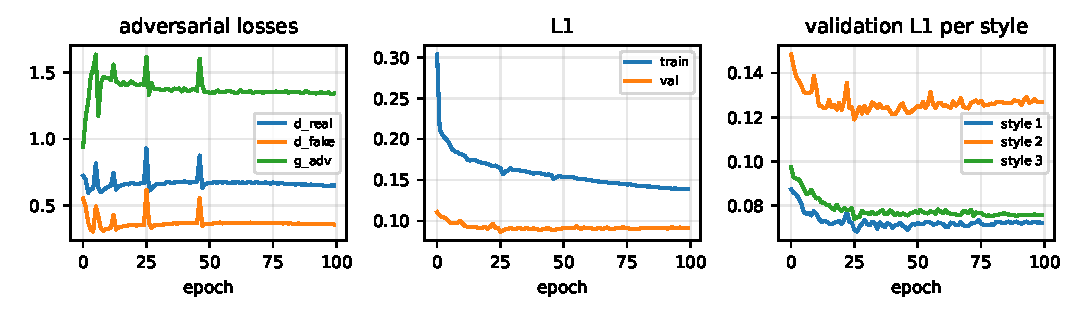
\includegraphics[width=\columnwidth]{t4_curves.pdf}\caption{Task 4 training curves (100 epochs).}\label{fig:t4curves}\end{figure}

\textbf{Test results.} Table~\ref{tab:t4} (1\,046 test pairs; the test set was never used for selection). Style~2 (dense cross-hatching) is by far the hardest (L1 0.146 vs.\ 0.075 for style~1); style~3 has only 46 test images. FID (102.1) is computed from 1\,046 images against 2\,048-d features and should be read only as a relative number. Fig.~\ref{fig:t4style} shows the same photographs under the three styles: Style~1 yields faint thin contours, Style~2 the darkest heavy strokes and Style~3 an intermediate weight, so the embedding controls stroke weight while identity is preserved, although the differences are modest compared with the very strong hatching of the ground-truth style~2/3 sketches.
\begin{table}[t]\centering\caption{Task 4 test metrics (FS2K official test set).}\label{tab:t4}\small
\begin{tabular}{@{}lccccc@{}}\toprule
Split & $n$ & L1 & SSIM & PSNR & LPIPS\\\midrule
Overall & 1046 & 0.1001 & 0.4983 & 16.14 & 0.382\\
Style 1 & 619 & 0.0750 & 0.5455 & 17.90 & 0.406\\
Style 2 & 381 & 0.1456 & 0.4057 & 12.90 & 0.354\\
Style 3 & 46 & 0.0614 & 0.6301 & 19.20 & 0.286\\\bottomrule
\end{tabular}\end{table}
\begin{figure}[t]\centering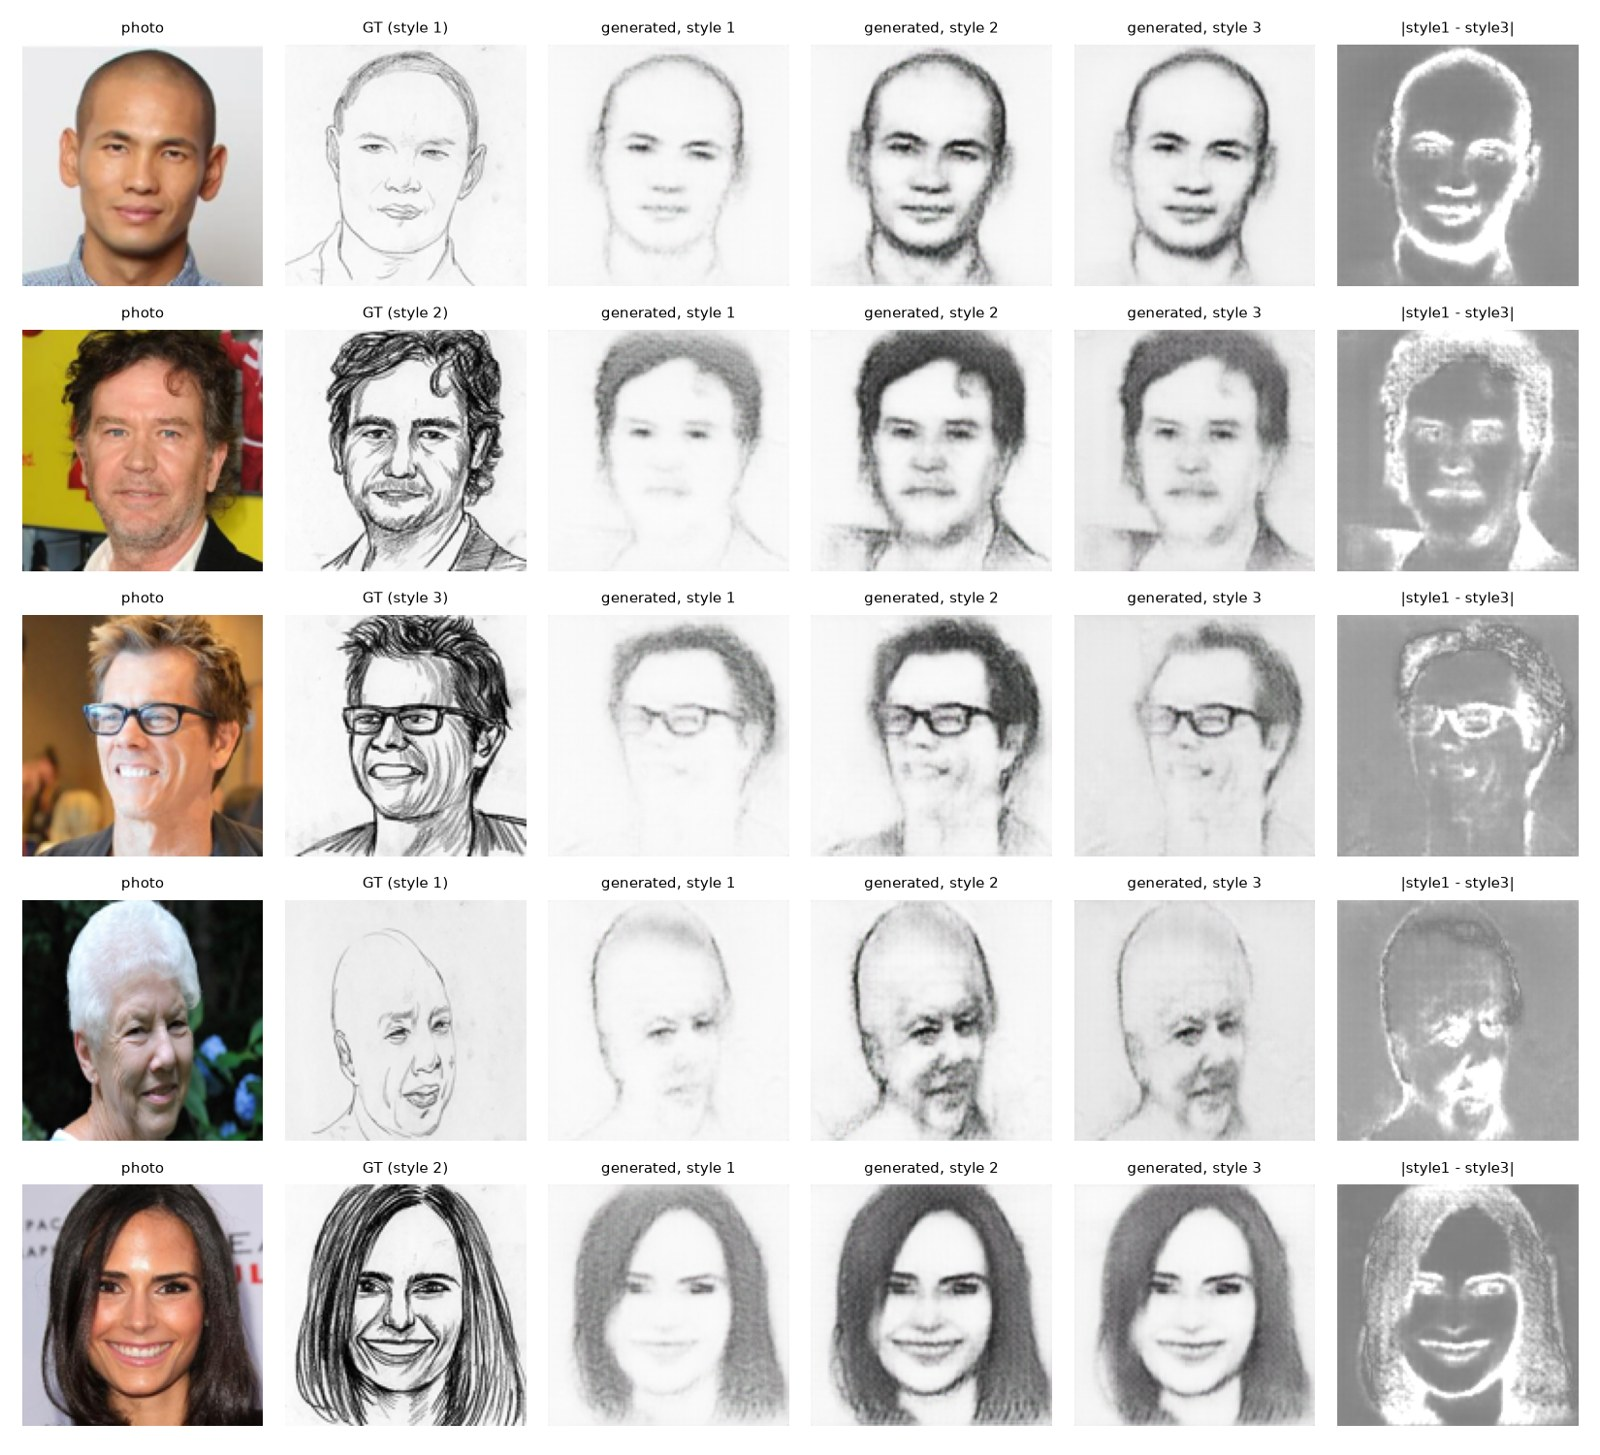
\includegraphics[width=\columnwidth]{t4_style_grid.jpg}\caption{Photo, ground truth and generated sketches for style 1/2/3 (last column: $|$style 1 $-$ style 3$|$).}\label{fig:t4style}\end{figure}
\begin{figure}[t]\centering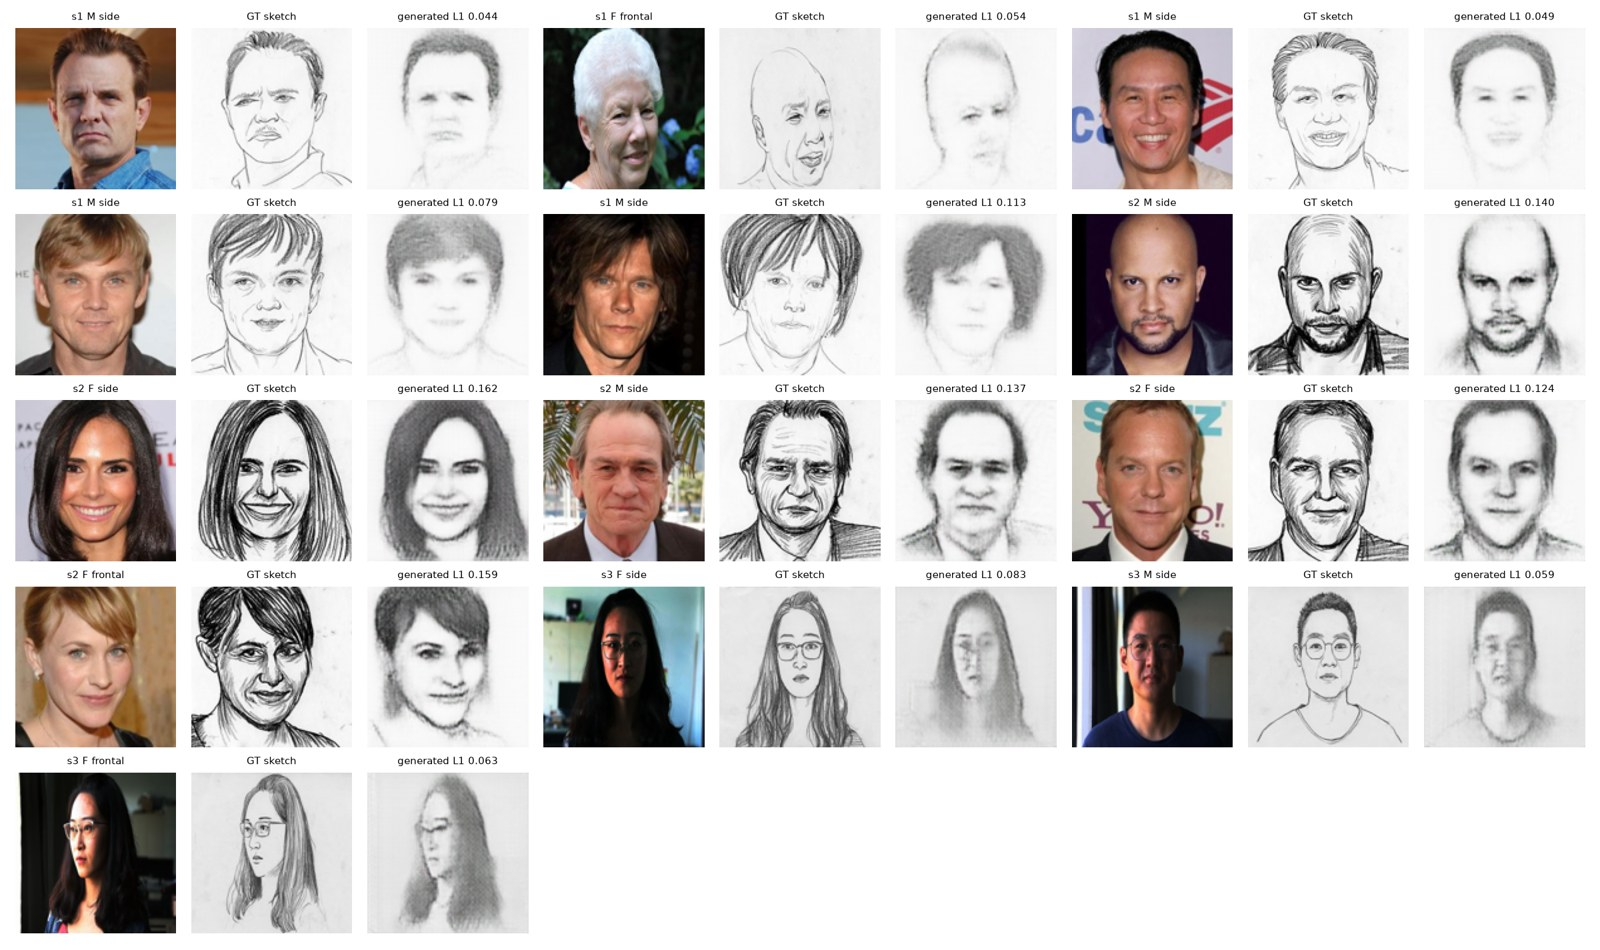
\includegraphics[width=\columnwidth]{t4_samples.jpg}\caption{Thirteen test examples (photo, ground truth, generation) across styles, gender and pose.}\label{fig:t4samples}\end{figure}
\textbf{Failure cases} (Fig.~\ref{fig:t4fail}; L1 0.23--0.30, SSIM 0.18--0.28): a side-lit woman with voluminous dark hair (hair becomes grey haze, expression lost), two style~2 women with long hair whose dense black ground-truth strokes are averaged into mid-grey texture, and a man in a peaked cap (hat and uniform collapse into a smudge). The L1-dominated objective on 899 training pairs regresses to the mean tone instead of committing to individual strokes, and rare accessories and non-frontal poses are under-represented.
\begin{figure}[t]\centering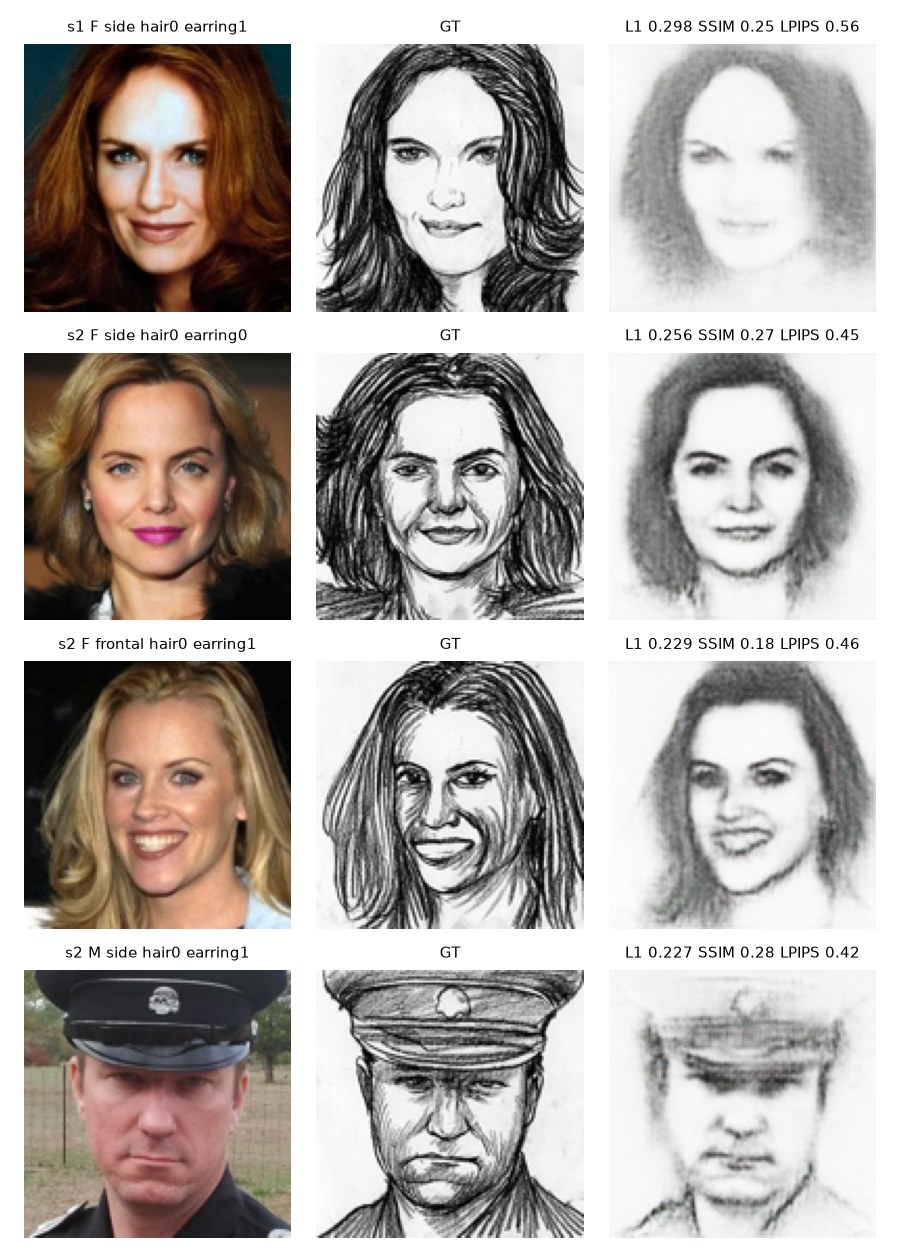
\includegraphics[width=0.85\columnwidth]{t4_failures.jpg}\caption{Task 4 failure cases (photo, ground truth, generated).}\label{fig:t4fail}\end{figure}

\section{Optimisation Summary, Export and Tracking}
All studies use SQLite-backed Optuna with TPE (seed 42) and a median pruner; Fig.~\ref{fig:optuna} shows trial values (the compute budget on a single 6\,GB GPU limited us to 10--12 trained trials per study, instead of the 30--50 originally planned). All runs log parameters, per-epoch metrics, sample grids and curves to MLflow (experiment names \texttt{genai-task\{N\}-*}; run names \texttt{trial-N}, \texttt{final}, \texttt{onnx-verify}). Models are exported with opset 17 and a dynamic batch axis and verified against PyTorch for batch sizes 1, 4, 8 (Table~\ref{tab:onnx}); our tolerance is $10^{-4}$ because $10^{-5}$ is below fp32 summation-order noise for the deepest network (observed maxima are lower).
\begin{figure}[t]\centering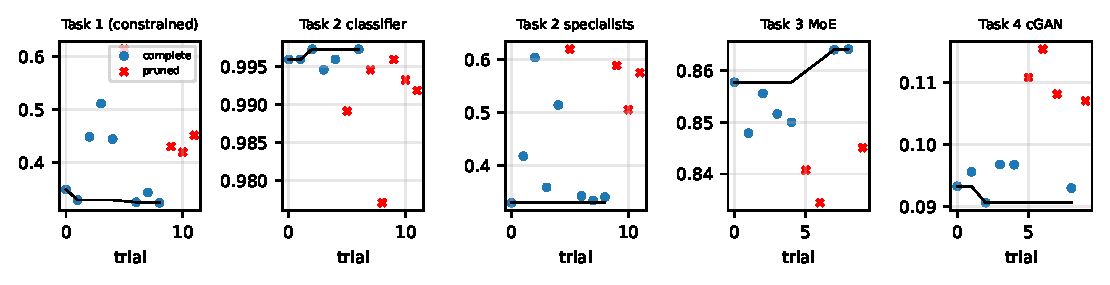
\includegraphics[width=\columnwidth]{optuna.pdf}\caption{Optuna trial values per study (circles: completed, crosses: pruned; line: best so far).}\label{fig:optuna}\end{figure}
\begin{table}[t]\centering\caption{ONNX export: maximum absolute difference to PyTorch and CPU latency (batch 1).}\label{tab:onnx}\small
\resizebox{\columnwidth}{!}{\begin{tabular}{@{}lccc@{}}\toprule
Model & size (MB) & max abs err & PyTorch$\to$ORT (ms)\\\midrule
Task 1 universal AE & 2.1 & $1.9\times10^{-5}$ & 14.0$\to$6.4\\
Task 2 classifier & 4.7 & $4.8\times10^{-6}$ & 14.4$\to$8.3\\
Task 2 specialists (3) & 2.1 each & $\le2.7\times10^{-6}$ & 13.9--14.9$\to$5.9--6.3\\
Task 3 soft MoE (single graph) & 10.9 & $1.5\times10^{-6}$ & 58.7$\to$28.7\\
Task 4 generator & 76.9 & $1.1\times10^{-6}$ & 45.1$\to$20.1\\\bottomrule
\end{tabular}}\end{table}

\section{Application Architecture}
The browser application has four workspaces (Universal Restoration, Hard-Routed Restoration, Soft Mixture-of-Experts Restoration, Face-to-Sketch Generator). The React/TypeScript/Tailwind single-page app is served by nginx, which also reverse-proxies \texttt{/api} and \texttt{/health} to a FastAPI backend (Fig.~\ref{fig:arch}). The backend validates uploads (JPEG/PNG only, $\le10$\,MB, decodable, sane dimensions; HTTP 400/413), preprocesses them to $128\times128$ tensors, runs ONNX Runtime sessions created once at start-up (CUDA if present, otherwise CPU), applies run-time corruptions with a NumPy re-implementation verified against the training code, and returns images as base64 PNG together with routing probabilities, gate weights, selected expert and timing (HTTP 503 with an actionable message if a model file is missing). The backend image is torch-free (pip with inference-only requirements). \texttt{docker compose up --build} starts both containers (backend health-checked before the frontend). Tests: 13 API tests on the real models, a 14-check live smoke test through nginx and an 8-step Playwright browser test whose screenshots appear in Fig.~\ref{fig:app}.
\begin{figure}[t]\centering
\resizebox{\columnwidth}{!}{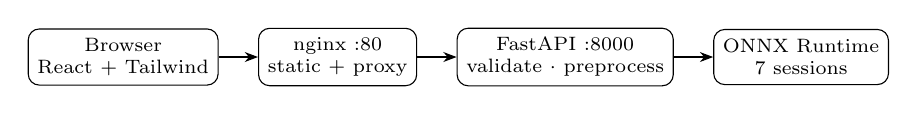
\begin{tikzpicture}[node distance=5mm,box/.style={draw,rounded corners,align=center,font=\scriptsize,minimum height=7mm},>=Stealth]
\node[box](b){Browser\\React + Tailwind};
\node[box,right=of b](n){nginx :80\\static + proxy};
\node[box,right=of n](f){FastAPI :8000\\validate $\cdot$ preprocess};
\node[box,right=of f](o){ONNX Runtime\\7 sessions};
\draw[->](b)--(n);\draw[->](n)--(f);\draw[->](f)--(o);
\end{tikzpicture}}\caption{Request path of the deployed application.}\label{fig:arch}\end{figure}
\textbf{Interface design (Google Stitch).} The layout, colours and components were first designed in Google Stitch (project \url{https://stitch.withgoogle.com/projects/16009442400636392007}) from a ``luminous glassmorphism'' brief: a peach--butter--periwinkle gradient, a large frosted-glass frame containing a floating icon navigation pill, glass bento cards, pill tabs and an amber/indigo accent pair (design tokens exported as \texttt{DESIGN.md}; Plus Jakarta Sans and Inter fonts). Fig.~\ref{fig:stitch} shows the four original Stitch screens (the exported screens and HTML are in \texttt{report/stitch/} of the repository). The Stitch mock-ups contain illustrative placeholder values (e.g.\ GPU names, a model name and a PSNR gauge); these were \emph{not} reproduced: the implemented React/Tailwind interface (Fig.~\ref{fig:app}) adopts the aesthetic and navigation structure but shows only values returned by the real models.
\begin{figure}[t]\centering
\includegraphics[width=\columnwidth]{stitch_design.jpg}\caption{Original Google Stitch design: Universal Restoration, Hard-Routed Restoration, Soft Mixture-of-Experts and Face-to-Sketch screens.}\label{fig:stitch}\end{figure}
\begin{figure}[t]\centering
\includegraphics[width=0.49\columnwidth]{app_universal.jpg}\hfill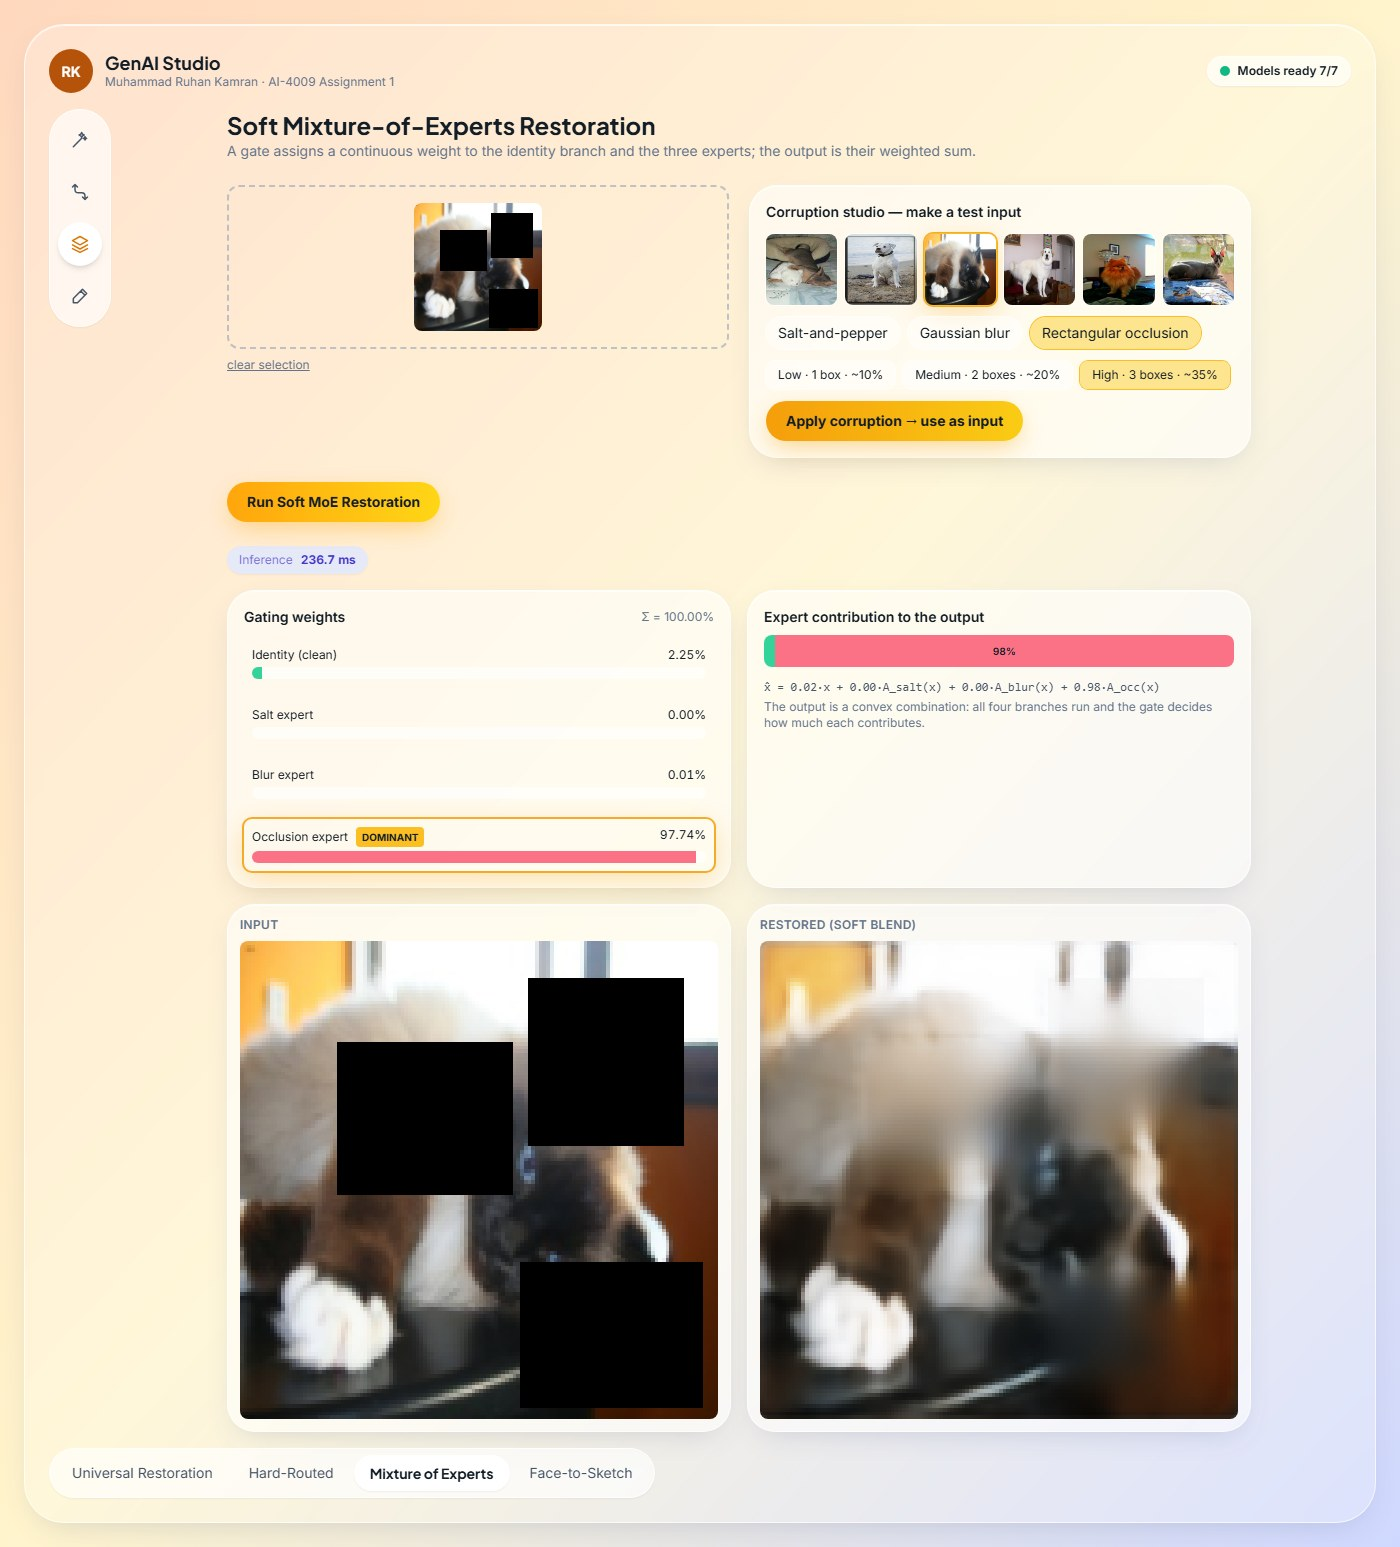
\includegraphics[width=0.49\columnwidth]{app_softmoe.jpg}\\[1mm]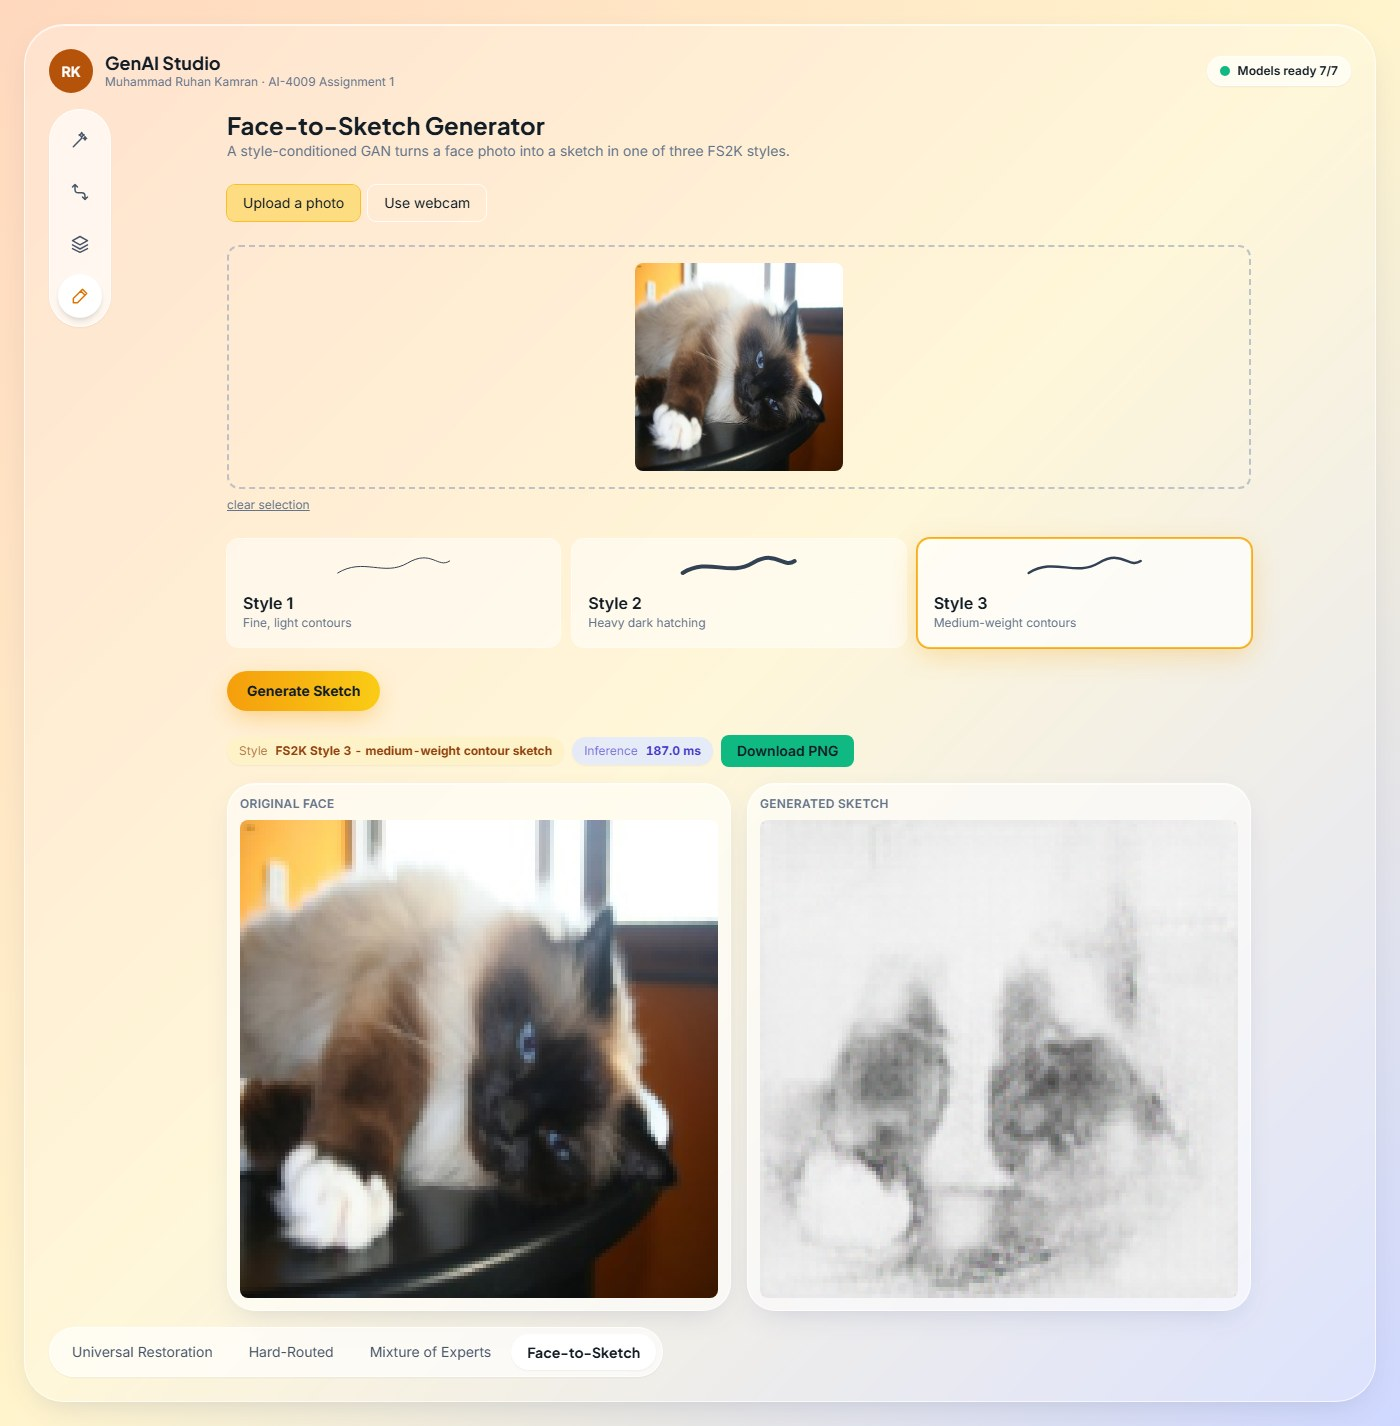
\includegraphics[width=0.49\columnwidth]{app_sketch.jpg}\caption{Implemented application (screenshots of the Docker deployment): Universal Restoration, Soft MoE and Face-to-Sketch.}\label{fig:app}\end{figure}

\section{Limitations and Conclusion}
\textbf{Limitations.} (i) Optuna budgets (10--12 trained trials per study, 5--20 epochs per trial) are much smaller than planned, so the selected configurations may be sub-optimal and several comparisons (classifier search, balance regularisers) are within noise; most design experiments use a single seed. (ii) The restoration models are blurry on high-frequency content and fail under large occlusions; no perceptual or adversarial term was used. (iii) The soft MoE cannot copy clean images exactly and its identity share hurts low-severity occlusion; its latency is 3.9$\times$ Task~1. (iv) The face-to-sketch outputs are softer than the ground truth; style~2 is weak; the style~3 test split has 46 images; FID is rank-deficient. (v) ResNet/attention U-Nets, AdaIN, multi-scale discriminators and a VGG perceptual loss were discussed but not run. (vi) The webcam path could not be exercised in the headless browser test.

\textbf{Conclusion.} Specialisation helps (+0.5\,dB) when routing is reliable, and a gate that blends experts gives a further gain (+0.5\,dB, +0.03 SSIM) with markedly better resilience to routing errors, at the price of exact-copy behaviour on clean inputs and 2$\times$ the latency. The full pipeline from data manifests to a containerised browser application is reproducible from the repository with one documented command.

\begin{thebibliography}{99}
\bibitem{vincent2008} P.~Vincent \emph{et al.}, ``Extracting and composing robust features with denoising autoencoders,'' in \emph{Proc. ICML}, 2008.
\bibitem{ronneberger2015} O.~Ronneberger, P.~Fischer, T.~Brox, ``U-Net: Convolutional networks for biomedical image segmentation,'' in \emph{MICCAI}, 2015.
\bibitem{wang2004} Z.~Wang \emph{et al.}, ``Image quality assessment: From error visibility to structural similarity,'' \emph{IEEE TIP}, vol.~13, no.~4, 2004.
\bibitem{shazeer2017} N.~Shazeer \emph{et al.}, ``Outrageously large neural networks: The sparsely-gated mixture-of-experts layer,'' in \emph{ICLR}, 2017.
\bibitem{fedus2021} W.~Fedus, B.~Zoph, N.~Shazeer, ``Switch Transformers: Scaling to trillion parameter models with simple and efficient sparsity,'' \emph{JMLR}, vol.~23, 2022.
\bibitem{mirza2014} M.~Mirza, S.~Osindero, ``Conditional generative adversarial nets,'' arXiv:1411.1784, 2014.
\bibitem{isola2017} P.~Isola \emph{et al.}, ``Image-to-image translation with conditional adversarial networks,'' in \emph{CVPR}, 2017.
\bibitem{perez2018} E.~Perez \emph{et al.}, ``FiLM: Visual reasoning with a general conditioning layer,'' in \emph{AAAI}, 2018.
\bibitem{akiba2019} T.~Akiba \emph{et al.}, ``Optuna: A next-generation hyperparameter optimization framework,'' in \emph{KDD}, 2019.
\bibitem{zhang2018} R.~Zhang \emph{et al.}, ``The unreasonable effectiveness of deep features as a perceptual metric,'' in \emph{CVPR}, 2018.
\bibitem{heusel2017} M.~Heusel \emph{et al.}, ``GANs trained by a two time-scale update rule converge to a local Nash equilibrium,'' in \emph{NeurIPS}, 2017.
\bibitem{parkhi2012} O.~M.~Parkhi \emph{et al.}, ``Cats and dogs,'' in \emph{CVPR}, 2012.
\bibitem{fan2022} D.-P.~Fan \emph{et al.}, ``Facial-sketch synthesis: A new challenge,'' \emph{Machine Intelligence Research}, 2022.
\end{thebibliography}
\end{document}
